\documentclass[11pt]{article}

% Packages
\usepackage[margin=1in]{geometry}
\usepackage{amsmath, amssymb}
\usepackage{enumitem}
\usepackage{booktabs}
\usepackage{fancyhdr}
\usepackage{titlesec}
\usepackage{xcolor}
\usepackage{mdframed}
\usepackage{array}
\usepackage{parskip}
\usepackage{graphicx}
\usepackage{float}

% Colors
\definecolor{darkblue}{RGB}{28, 56, 96}
\definecolor{lightgray}{RGB}{245, 245, 245}
\definecolor{rulegray}{RGB}{180, 180, 180}

% Page style
\pagestyle{fancy}
\fancyhf{}
\rhead{\small ECE 370 - Midterm 2 Formula Sheet}
\lhead{\small Chapters 5 \& 6}
\rfoot{\small Page \thepage}
\renewcommand{\headrulewidth}{0.4pt}
\renewcommand{\footrulewidth}{0.4pt}

% Question counter
\newcounter{qnum}
\newcommand{\question}[2]{%
  \stepcounter{qnum}%
  \vspace{10pt}%
  \noindent\textbf{Question \theqnum} \\ \\ 
  \noindent #2%
  \vspace{4pt}%
}

% Sub-parts
\newlist{parts}{enumerate}{1}
\setlist[parts]{label=(\alph*), leftmargin=1.5em, topsep=4pt, itemsep=2pt}

% Vectors
\renewcommand{\vec}[1]{\mathbf{#1}}
\newcommand{\xhat}{\hat{\mathbf{x}}}
\newcommand{\yhat}{\hat{\mathbf{y}}}
\newcommand{\zhat}{\hat{\mathbf{z}}}
\newcommand{\rhat}{\hat{\mathbf{r}}}
\newcommand{\phihat}{\hat{\boldsymbol{\phi}}}

% ============================================================
\begin{document}

\begin{mdframed}[backgroundcolor=lightgray, linecolor=rulegray]
\small\textbf{Useful Constants:}\\[4pt]
Free space permeability: $\mu_0 = 4\pi \times 10^{-7}$ H/m \hfill Free space permittivity: $\varepsilon_0 = 8.854 \times 10^{-12}$ F/m \hfill \\[4pt]
\small\textbf{Chapter 1:}\\[4pt]
\centerline{Euler's Identity: $e^{j\theta} = \cos{\theta} + j\sin{\theta}$}\\[4pt] \centerline{Rectangular to polar: $x=|z|\cos{\theta}$,\quad$y=|z|\sin{\theta}$,\quad$|z|=\sqrt{x^2+y^2}$,\quad$\theta=\tan^{-1}(y/x)$}\\[4pt]
\small\textbf{Chapter 3:}\\[4pt]
Dot product: $\vec{A}\cdot \vec{B} = AB\cos\theta_{AB}$ \hfill Cross product: $\vec{A} \time \vec{B} = \mathbf{\hat{n}}AB\sin{\theta_{AB}}$\quad or \quad \begin{vmatrix}\mathbf{\hat{x}} & \mathbf{\hat{y}} & \mathbf{\hat{z}} \\ A_x & A_y & A_z \\ B_x & B_y & B_z \end{vmatrix}\\[4pt]
\small\textbf{Chapter 5:}\\[4pt]
Ampere's law: $\oint_C \vec{H} \cdot d \vec{l} = I$ \hfill Lorentz force: $\vec{F} = q(\vec{E} + \vec{u} \times \vec{B})$ \hfill Magnetic Gauss's: $\oint_S \vec{B} \cdot d \vec{s} = 0$ \\[4pt] Torque: $\vec{T} = \vec{m} \times \vec{B}$ \hfill Moment: $\vec{m} = \hat{n}NIA$ \hfill Biot-Savart: $\vec{H} = \frac{I}{4\pi}\int_l \frac{d \vec{l} \times \hat{R}}{R^2}$ \\[4pt] \hfill Infinite Wire: $\vec{B} = \hat{\phi} \frac{\mu_0I}{2\pi r}$ \hfill Circular Loop: $\vec{H} = \hat{z}\frac{Ia^2}{2(a^2+z^2)^{3/2}}$ \hfill Solenoid: $\vec{B} \approx \hat{z} \mu n I = \frac{\hat{z}\mu N I}{l}$ \hfill \\[4pt]
Inductance: $L = \frac{\Lambda}{I} = \frac{\Phi}{I} = \frac{1}{I}\int_S \vec{B} \cdot d \vec{s}$\hfill
Boundary conditions: $H_{1t} - H_{2t} = J_s$,\quad$B_{1n} = B_{2n}$\\[4pt]
\small\textbf{Chapter 6:}\\[4pt]
\centerline{Faraday's Law: $V_\text{emf} = -\dfrac{d\Phi}{dt} = \frac{d}{dt}\int_S \vec{B} \cdot d \vec{s} = V^{\mathrm{tr}}_{\mathrm{emf}}+V^{\mathrm{m}}_{\mathrm{emf}}$}\\[4pt]
$V^\text{tr}_\text{emf} = -N \int \frac{\partial \vec{B}}{\partial t} \cdot d \vec{s} \hfill V^\text{m}_\text{emf} = $\oint_C(\vec{u} \time \vec{B}) \cdot d \vec{l}$\\[4pt]
\end{mdframed}
\begin{figure}[H]
  \centering
  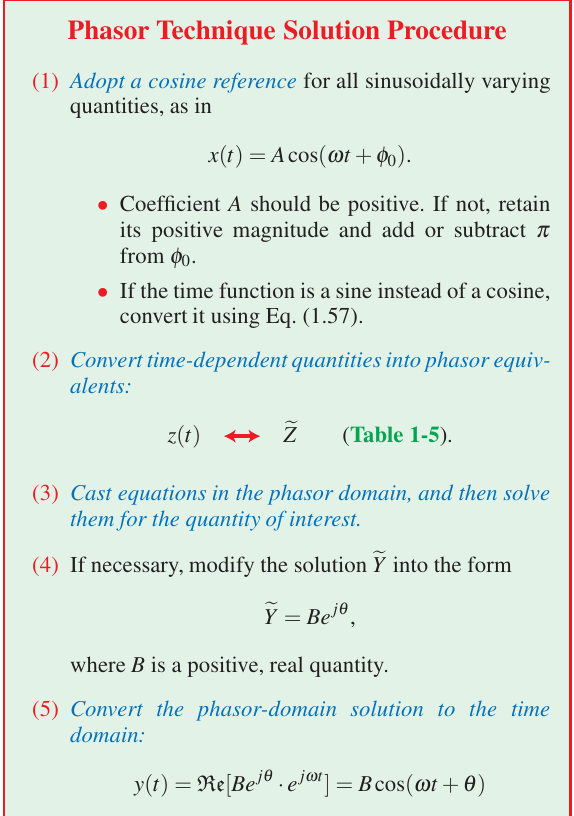
\includegraphics[width=0.4\textwidth]{formula-sheet_fig-4.png}
  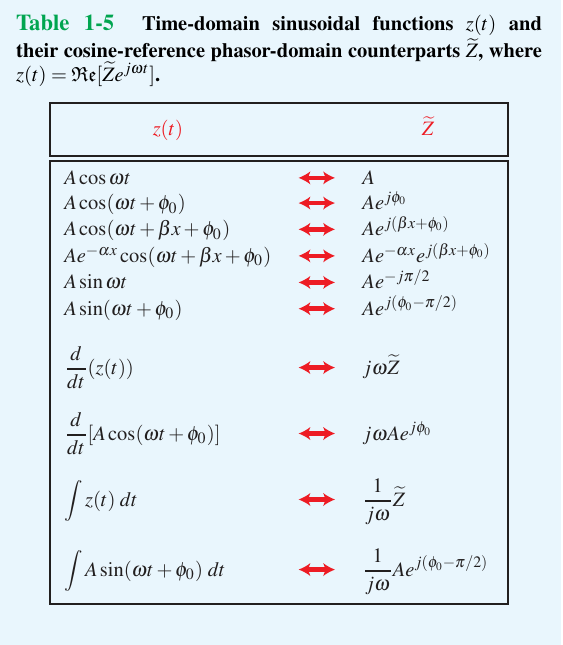
\includegraphics[width=0.5\textwidth]{formula-sheet_fig-3.png}
\end{figure}
\begin{figure}[H]
  \centering
  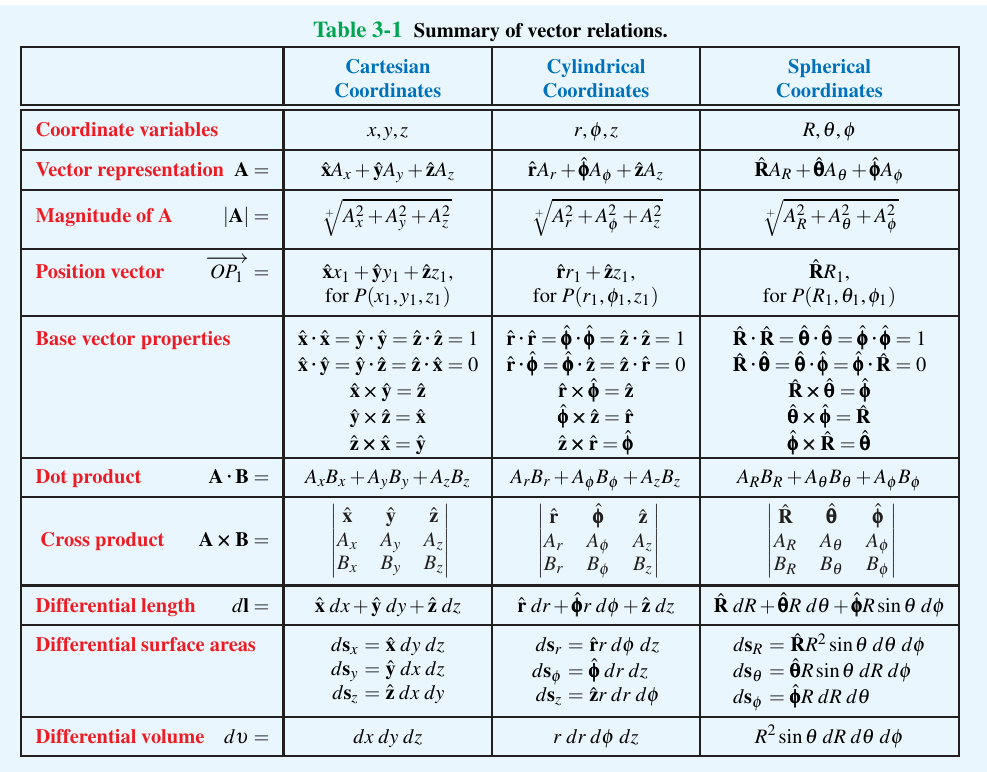
\includegraphics[width=0.8\textwidth]{formula-sheet_fig-1.png}
\end{figure}
\begin{figure}[H]
  \centering
  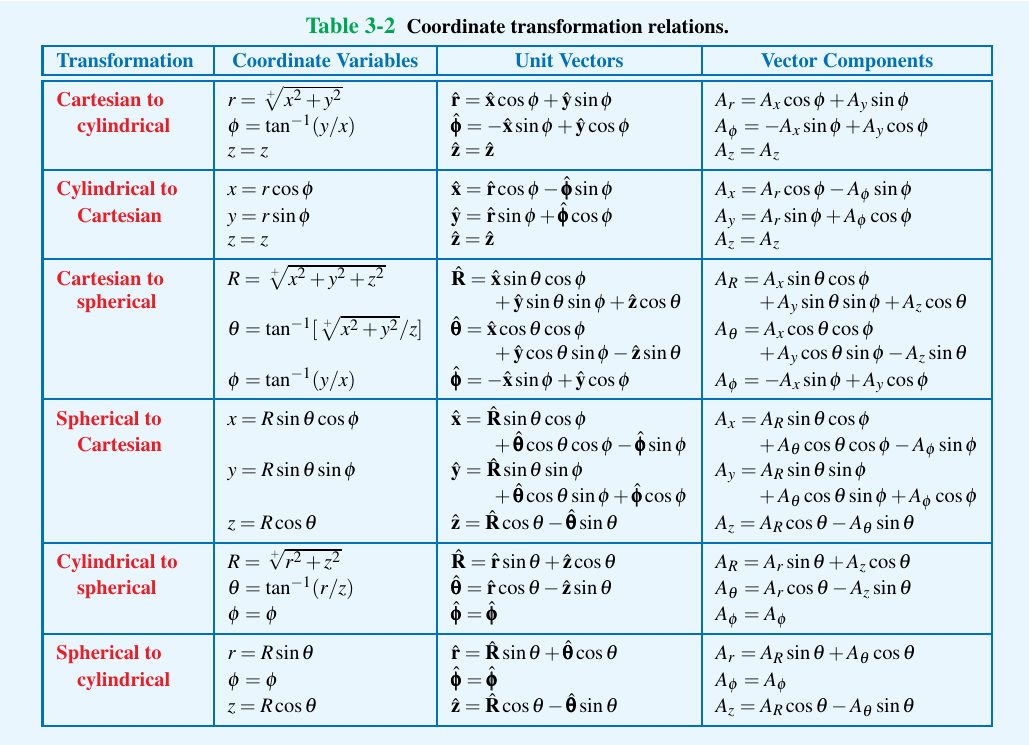
\includegraphics[width=0.8\textwidth]{formula-sheet_fig-2.png}
\end{figure}
\end{document}
